\section{Introduction}
The Antarctic Impulsive Transient Antenna (ANITA) experiment is a NASA-funded, balloon-borne experiment aiming primarily to detect Ultra-High-Energy (UHE) neutrinos and cosmic rays~\cite{ANITA1detector,ANITA1paper,ANITA2paper,ANITA2erratum}.
UHE neutrinos may be produced when cosmic rays interact with the
cosmic microwave background, either through the Greisen Zatsepin
Kuzmin (GZK)~\cite{greisen1966end,zatsepin1966gt} mechanism or through photo-disintegration; or directly from an astrophysical source.
UHE neutrinos interact in the Antarctic ice and produce a coherent radio pulse of Askaryan radiation~\cite{askaryan}. UHE cosmic rays interact with the geomagnetic field to produce a coherent radio impulse~\cite{ANITA1UHECR}. The geometry of the Earth's magnetic field in Antarctica allows ANITA to distinguish the signatures of these two types of events through their polarization.

The ANITA experiment flies approximately 40\,km above Antarctica looking for radio signals in the band between 200 and 1200\,MHz, produced by UHE neutrinos and cosmic rays.
Figure~\ref{fig:intro_ANITAconcept} shows a basic scheme of the
Askaryan neutrino detection at the ANITA experiment, as well as the UHE cosmic ray detection principle.
Four ANITA flights (Section~\ref{sec:anita3}) have been successfully completed so far, and this paper focuses on the simulations of the third and fourth ANITA flights.

\begin{figure}[!h]\centering
  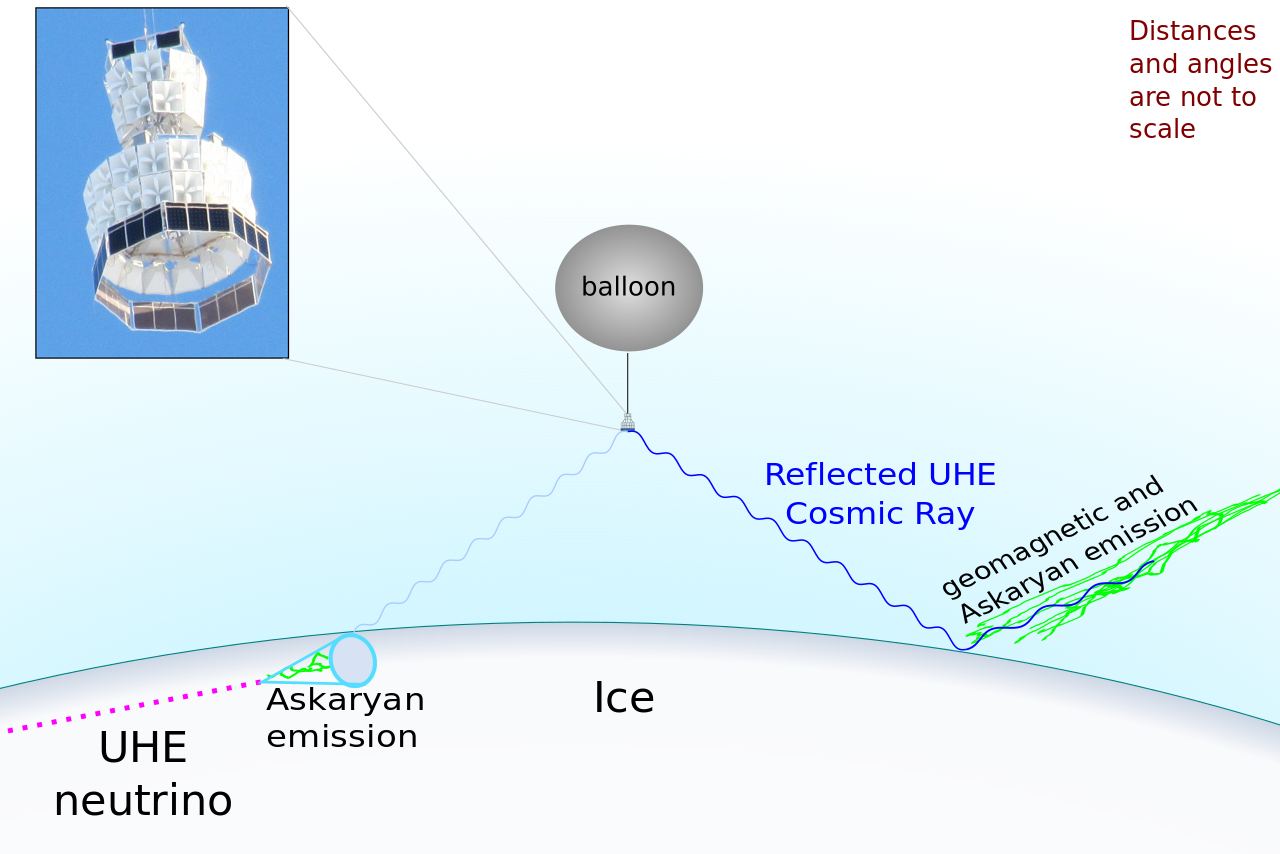
\includegraphics[width=.8\linewidth]{./Figs/ANITA_scheme_icemcpaper.png}
  \caption{The ANITA detection concept with a photo of the ANITA-IV payload. UHE neutrinos interact with the Antarctic ice and produce a coherent radio pulse of Askaryan radiation. UHE cosmic ray interactions in the atmosphere produce a shower of secondary particles that interact with the geomagnetic field to produce a coherent radio impulse. These signals are detected by the ANITA instrument, given its position on a NASA long duration balloon. %\CD{Since the paper isn't really about CR's, is it worth discussing them?}
  }
  \label{fig:intro_ANITAconcept}
\end{figure}



The \icemc program is a C++ Monte Carlo simulation tool based on
ROOT~\cite{brun1997root} used to simulate UHE neutrino interactions producing Askaryan radiation. 
This tool is used by the ANITA collaboration to tune the neutrino
analysis selection and quantify the experiment's sensitivity.


\begin{figure}[!h]\centering
  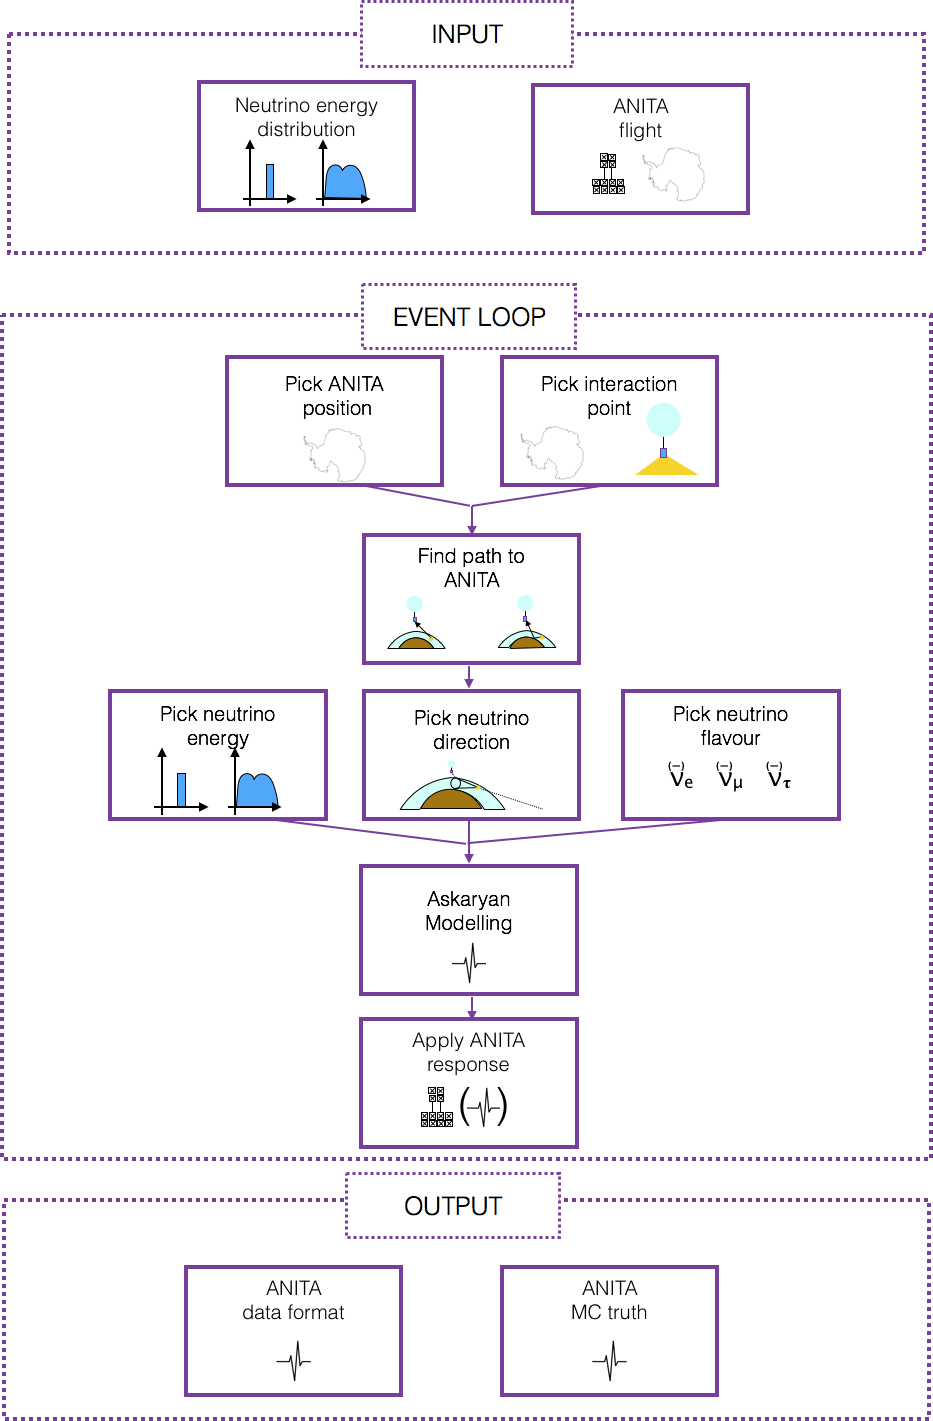
\includegraphics[width=.8\linewidth]{./Figs/IcemcFlowchart.png}
  \caption{Flowchart of the \icemc simulation for a single candidate.}
  \label{fig:intro_icemcFlow}
\end{figure}

A flowchart of the \icemc simulation steps is shown in Figure~\ref{fig:intro_icemcFlow}.
%The simulation models neutrino interactions in the ice from a specific energy or following a theoretical energy spectrum.
At the beginning of each run the user can choose which ANITA flight to simulate and which neutrino energy spectrum to use.
For each neutrino event, the position along the ANITA flight path, as well as the neutrino interaction position are randomly chosen.
These are used to find the path to the ANITA detector (Section~\ref{sec:eventGeometry}).% and used to calculate the event weight.
%The restrictions in neutrino phase space  that arise in the selection of the neutrino interaction positions and neutrino directions are corrected for in the final calculation (see Section~\ref{sec:weights}).
The neutrino direction is then chosen within allowed angles; the neutrino energy is chosen following the input theoretical model; and the neutrino flavour and interaction type are chosen according to their expected ratio. 
These parameters are used to produce the radio frequency pulse following the Askaryan model described in Section~\ref{sec:rf}.
The signal is then propagated through the ice and air to the ANITA
detector (see Section~\ref{sec:propagation}). 
The response of the ANITA signal chain is simulated, and the resulting 
data are saved in the same format as ANITA flight data 
(see Section~\ref{sec:ANITA}).
Different parts of the simulation are validated against data taken both in
the lab and in-flight during the past ANITA flights (see
Section~\ref{sec:validation}).
Finally the neutrino acceptance of the third and fourth ANITA flight is
presented, and how the uncertainties in the different parts of the
simulation impact the acceptance (see Section~\ref{sec:results}).



%\section{Motivation}

\section{The ANITA flights}
\label{sec:anita3}
The first two ANITA payloads flew in 2006-2007\cite{ANITA1paper} and 2008-2009\cite{ANITA2paper,ANITA2erratum}, respectively.
Although \icemc can be used to simulate older flights, this paper focusses on the simulation of the third and fourth flights.
The third ANITA payload (ANITA-III) launched on December 18$^{\text{th}}$, 2014 from the
NASA Long Duration Balloon (LDB) facility near McMurdo Station, Antarctica.
ANITA-III followed the polar vortex flying at the altitude of 37\,km for
22 days until January 9$^{\text{th}}$, 2015 when the flight was terminated
near Australian Davis Station.
Similarly, the fourth ANITA payload (ANITA-IV) launched on December 2$^{\text{nd}}$, 2016 from the NASA LDB facility in Antarctica and landed approximately 100\,km from the South Pole Station on December 29$^{\text{th}}$, 2016.
Figure~\ref{fig:ANITA_flightPath} shows the flight paths of the ANITA-III and ANITA-IV instruments. 
The colormap shows the Antarctic ice depth.

\begin{figure}[!h]\centering
  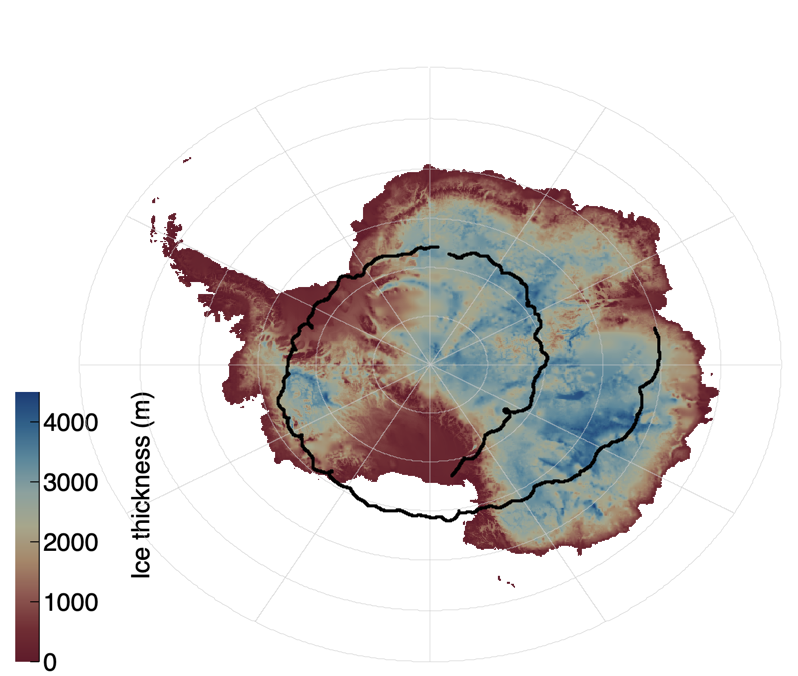
\includegraphics[width=.45\linewidth]{./Figs/Flightpath_ANITA3.png}
  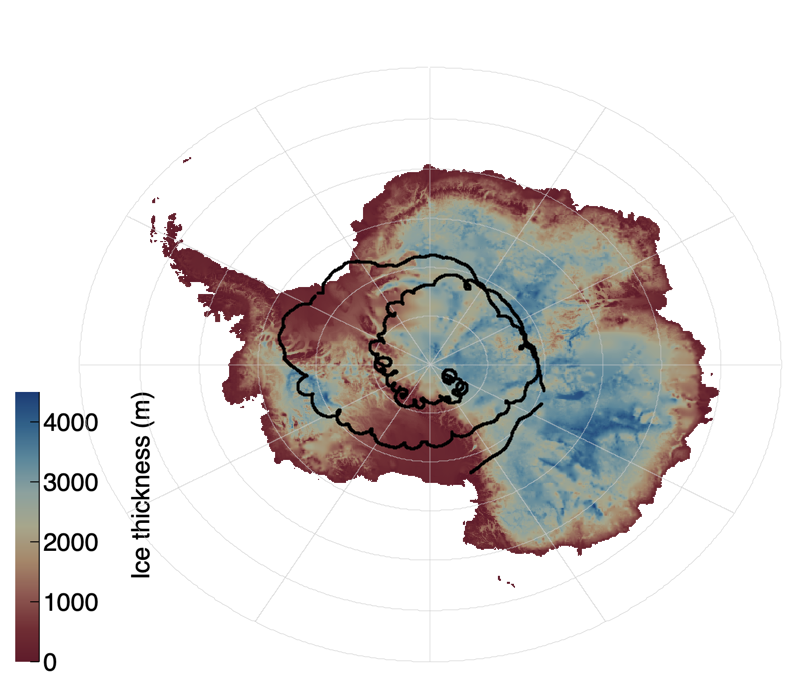
\includegraphics[width=.45\linewidth]{./Figs/Flightpath_ANITA4.png}
  \caption{Flight path simulated in \icemc for the ANITA-III (left) and ANITA-IV (right) flights.
    Antarctica map produced using the BEDMAP model~\cite{bedmap}.     }
  \label{fig:ANITA_flightPath}
\end{figure}



\begin{figure}[!h]\centering
  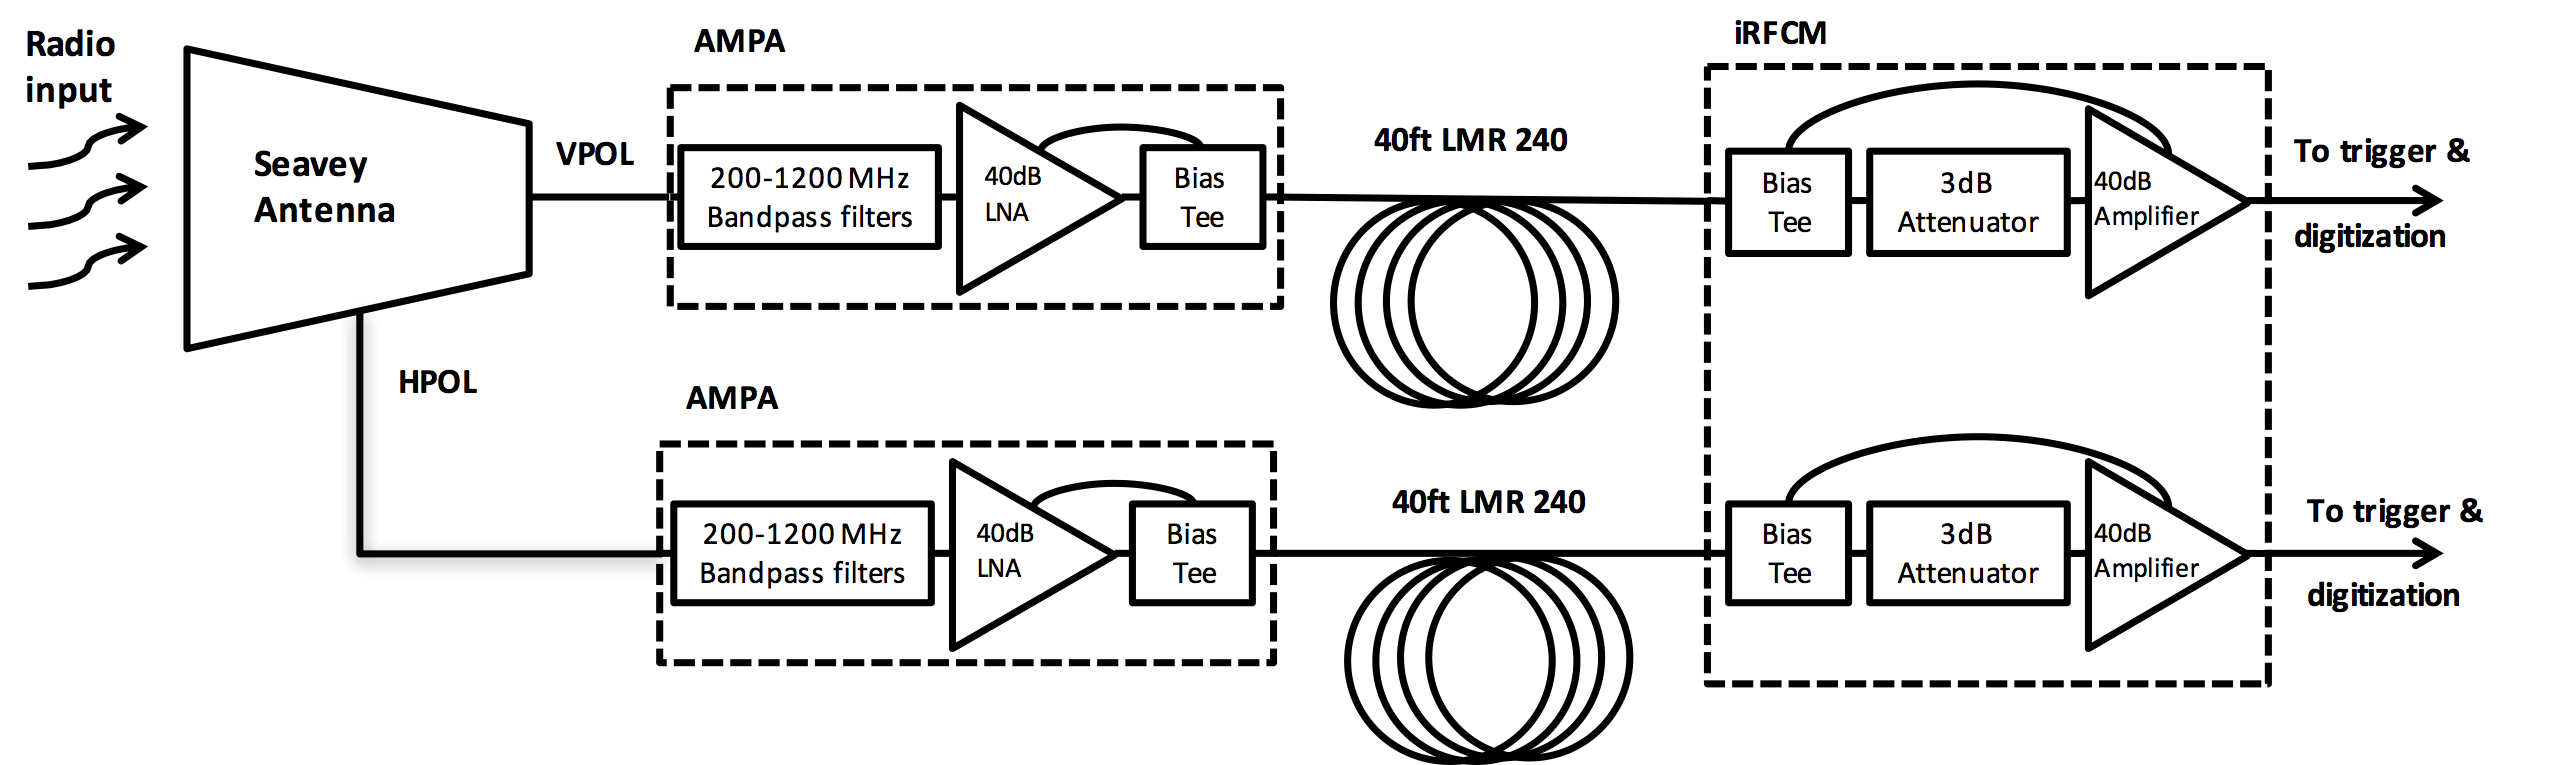
\includegraphics[width=.95\linewidth]{./Figs/ANITA3_signalChain1.png}
  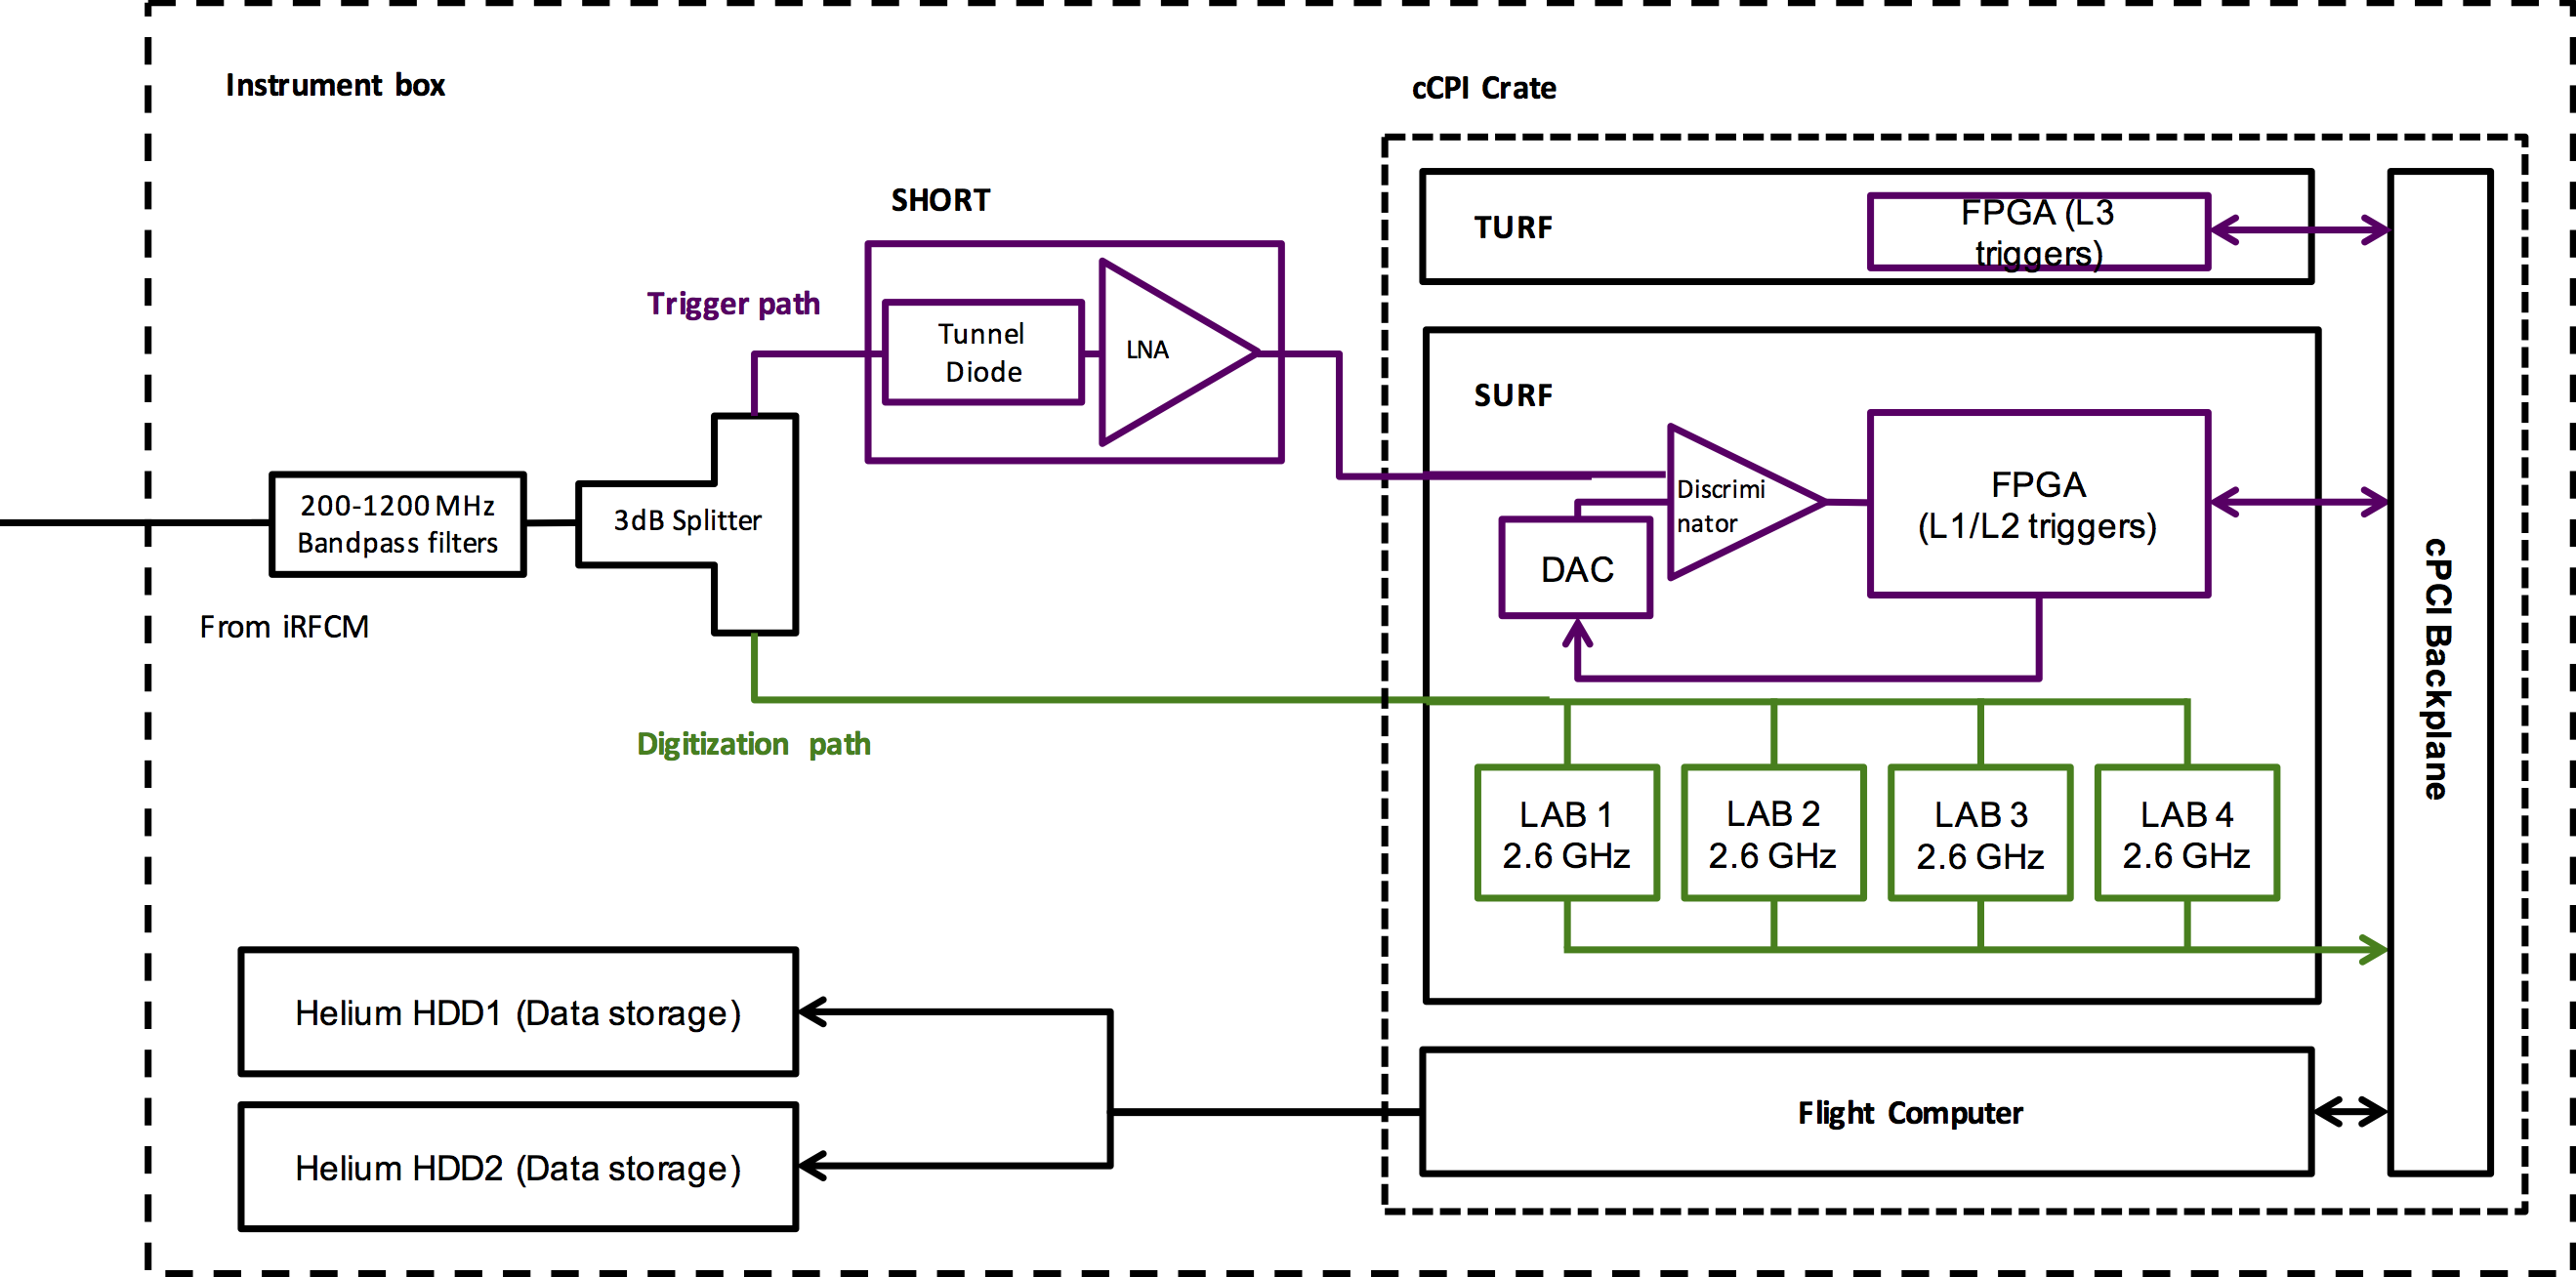
\includegraphics[width=.95\linewidth]{./Figs/ANITA3_signalChain2.png}
  \caption{ANITA-III signal chain.
  The receiving antenna splits signals into vertical and horizontal
  polarizations which follow identical paths. 
After going through filters and amplifiers, the signal is split into
the trigger and digitizer paths. In the trigger path the signal passes
through a tunnel diode and is compared to a threshold. 
When a trigger is issued, a switched capacitor array digitizes the
signal with a mean sample rate of 2.6\,GSa/s.}
  \label{fig:ANITA3_signalChain}
\end{figure}


The ANITA-III and ANITA-IV instruments were similar to the two previous
ones~\cite{ANITA1paper,ANITA2paper}, using 48 dual polarization quad-ridged horn antennas with bandwidth from 200 to 1200\,MHz (ANITA-I had 32 and ANITA-II had 40). 
The antennas were arranged in three rings forming 16 azimuthal sectors per ring (the top ring is divided into two layers to fit into the launch envelope specifications), as shown in Figure~\ref{fig:intro_ANITAconcept}.

Figure~\ref{fig:ANITA3_signalChain} shows a schematic of the ANITA-III signal chain. 
The receiving antenna measures vertical and horizontal polarization signals of incident radio waves, which then follow twin paths. 
After passing through filters and amplifiers, the signal is split into
the trigger and digitizer paths.
In the trigger path the signal passes
through a tunnel diode which acts as a square-law detector over the
input range. The output of the tunnel diode is compared to the channel
threshold, which is dynamically adjusted by a PID loop to maintain a desired 
rate for each antenna. A combination of first-level and second-level triggers forms a
global trigger which can be issued in each polarization.
When a trigger is issued, a switched capacitor array digitizes the signal with a mean sample rate of 2.6\,GSa/s. 
The ANITA-IV signal chain included the Tunable Universal Filter Frontend boards (see Subsection~\ref{subsec:tuffs}), and $90^{\circ}$ hybrids to convert the signal into left- and right- circularly polarized (LCP and RCP) components. 
The ANITA-IV trigger logic also required a coincidence between LCP and RCP signals within a 4\,ns coincidence window, implying a linear polarization requirement on the trigger. 

As the payload rotates freely, two sets of GPS units were used to independently determine the
payload position and attitude.
Power was supplied by an octagonal array of photovoltaic panels and stored using four pairs of 12-V lead-acid batteries.
Communication to and from the payload was through the Iridium and TDRSS satellite systems throughout the flight, and by a direct line-of-sight radio link when within range of McMurdo Station.

%\section{Overall Strategy}
%\label{sec:strategy}
%\todo[inline]{Add integral of what we want to calculate, with all the parts of what we need, and relate to sections Acceptance}

%We require an interaction to occur within
%the Antarctic ice volume within the balloon horizon.  
%We generate two different types of events.  The first is where the
%ray seen by the balloon is direct; the ray is emitted from the
%interaction upward.  The second is where the ray is emitted downward
%and is reflected from the ice-rock interface before reaching
%the surface.  For half of the neutrinos, we force the ray to be the
%first type and for the other half, the second type.
%For a given type of ray, we find the unique path along which
%an RF signal would travel from the interaction to the balloon, snelled
%through ice layers at the ice-air surface.  

%Next, we pick a direction for the neutrino
%path, only considering directions such that the Cherenkov cone is
%close enough to the unique ray from interaction to balloon that
%the signal is still detectable under a best-case scenario.
%Depth-dependent attenuation lengths and indexes of refraction
%in the ice are based on recent South Pole measurements[CITE].  
%Surface slopeyness is taken into account under a simple model.

%The ANITA instrument response is based on measurement made in
%Antarctica prior to the flights, and the system noise is simulated
%according to measurements performed during the flight.
%The trigger configuration is based on the most
%current design.


